%% GCM 2026
%% https://conf.researchr.org/home/staf-2026/gcm-2026#Call-for-Papers
%% Regular papers of at most 16 pages describing innovative contributions.
%% Position papers, system descriptions or work in progress of 6 to 12 pages.



%% The first command in your LaTeX source must be the \documentclass command.
%%
%% Options:
%% twocolumn : Two column layout. Do not use twocolumn for papers submitted to CEUR-WS!
%% hf: enable header and footer.
\documentclass[
% twocolumn,
% hf,
]{ceurart}

%%
%% One can fix some overfulls
\sloppy

%%
%% Minted listings support 
%% Need pygment <http://pygments.org/> <http://pypi.python.org/pypi/Pygments>
\usepackage{listings}
%% auto break lines
\lstset{breaklines=true}
\usepackage{amsthm}
\newtheorem{definition}{Definition}
\usepackage{minted}

\usepackage{wrapfig}

\usepackage{tikz}
\usepackage{tikz-inet}
\usetikzlibrary{positioning, arrows.meta, patterns, calc}
\usepackage{subcaption}
\usepackage{xcolor}
\colorlet{darkred}{red!60!black}
\colorlet{darkblue}{blue!60!black}
\colorlet{darkgreen}{green!60!black}


%%
%% end of the preamble, start of the body of the document source.
\begin{document}

%%
%% Rights management information.
%% CC-BY is default license.
\copyrightyear{2022}
\copyrightclause{Copyright for this paper by its authors.
  Use permitted under Creative Commons License Attribution 4.0
  International (CC BY 4.0).}

%%
%% This command is for the conference information
\conference{Woodstock'22: Symposium on the irreproducible science,
  June 07--11, 2022, Woodstock, NY}

%%
%% The "title" command
%\title{Graph Analysis via Graph Rewriting: Sparse Linear Algebra Based Graph Analysis in Interaction Nets}
\title{Preliminary Study of Interaction Nets Applicability for Sparse Linear Algebra Based Graph Analysis}

%%
%% The "author" command and its associated commands are used to define
%% the authors and their affiliations.
\author[1]{Danil Zaripov}[%
orcid=0009-0003-1086-9279,
email=st129060@student.spbu.ru,
]
\cormark[1]

\author[1]{Efim Kubyshkin}[%
orcid=0009-0009-5531-1758,
email=e.kubyshkin@spbu.ru,
]

\author[1]{Nikolai Ponomarev}[%
orcid=0009-0000-2382-5687,
email=n.ponomarev@spbu.ru,
]

\author[1]{Georgy Sichkar}[%
orcid=0009-0005-4684-9610,
email=georgy.sichkar@yandex.ru,
]

\author[1]{Vladimir Zaikin}[%
orcid=0009-0003-3417-990X,
email=st119057@student.spbu.ru,
]

\author[1]{Semyon Grigorev}[%
orcid=0000-0002-7966-0698,
email=s.v.grigoriev@mail.spbu.ru,
]
\cormark[1]


\address[1]{Saint Petersburg State University,
  7-9 Universitetskaya Embankment, St. Petersburg, 199034, Russia}



%% Footnotes
\cortext[1]{Corresponding author.}

%%
%% The abstract is a short summary of the work to be presented in the
\begin{abstract}
%% article.
  Developing scalable parallel algorithms for graph analysis remains challenging due to the irregular nature of graphs, which makes load balancing non-trivial.
  Interaction Nets naturally support irregular parallelism at a low level, making them a promising foundation for graph analysis.
  Using two Interaction Net implementations, Vine and Inpla, we provided an equivalent set of primitives and functions over quad-tree-represented matrices and vectors, and conducted a preliminary performance evaluation.
  From this, we derived several observations regarding Vine and Inpla, along with directions for future research.
\end{abstract}

%%
%% Keywords. The author(s) should pick words that accurately describe
%% the work being presented. Separate the keywords with commas.
\begin{keywords}
  Interaction Nets \sep
  graph rewriting \sep
  graph analysis algorithms \sep
  GraphBLAS \sep
  sparse linear algebra \sep
  quad-tree
\end{keywords}

%%
%% This command processes the author and affiliation and title
%% information and builds the first part of the formatted document.
\maketitle

\section{Introduction}

Graph analysis has become fundamental to modern data science, powering applications ranging from recommendation systems in social networks and fraud detection in financial transactions to protein interaction analysis in bioinformatics and static code analysis.
As graph sizes grow to billions of vertices and edges, the need for efficient, scalable implementations becomes critical.
However, graph analysis algorithms are difficult to parallelize due to their irregular memory access patterns, poor data locality, and load imbalance across computational units.

%The GraphBLAS standard~\cite{9460572} addresses these challenges by providing a foundation for constructing high-performance parallel graph analysis algorithms.
%By expressing graph algorithms in the language of linear algebra~--- using generic sparse vectors and matrices as core data structures, together with a rich set of highly parameterizable operations (matrix multiplication, element-wise operations, etc.)~--- GraphBLAS offers a high-level, mathematically rigorous framework for algorithm construction.
%Operations over sparse generic matrices and vectors parameterized by semiring-like structures provide a powerful basis for expressing a wide range of graph analysis algorithms~\cite{8778338}.
%
%Despite its successes, GraphBLAS and its implementations face certain challenges including the implementation of high-performance generic operations over sparse data structures.
%Imbalanced subtasks together with irregular data access patterns make load balancing~--- and thus efficient parallel implementation~--- hard.
%Moreover, graph analysis algorithms are not single operations but nontrivial chains of operations over matrices and vectors.
%This leads to the problem of intermediate data structures.
%Kernel fusion could solve these problems, but it is too difficult to implement automatic optimizations for sparse generic computations, so it is done manually in the most frequent cases.

The GraphBLAS standard~\cite{9460572} addresses these challenges by providing a foundation for high-performance parallel graph analysis, expressing algorithms in linear algebra using generic sparse vectors/matrices and parameterizable operations. However, implementing high-performance generic operations over sparse data remains challenging: irregular access and imbalanced subtasks complicate load balancing and parallelization, while nontrivial chains of operations create intermediate data structures. Kernel fusion could help, but automatic optimization for sparse generic computations is difficult, so it is performed manually in the most common cases.

At the same time, Interaction Nets~\cite{10.1145/96709.96718}~--- a graph-rewriting model introduced by Yves Lafont~--- offer a computational model that is inherently well-suited for irregular parallelism.
In Interaction Nets, computation proceeds through local rewriting rules applied to pairs of connected nodes (so-called active pairs).
Crucially, multiple non-interfering active pairs can be reduced simultaneously, making Interaction Nets a promising foundation for parallel irregular computations, including graph analysis.
Furthermore, Interaction Nets are relatively close to functional programming languages, making it easy to transfer design approaches and ideas from the functional world.

However, comparisons between existing interaction-net-based evaluators remain very limited and are often performed only on basic benchmarks such as Fibonacci, Ackermann, sorting, and list traversal.

We believe that Interaction Nets can provide a powerful foundation for implementing graph analysis algorithms.
The long-term goal of our work is to investigate how Interaction Nets can help solve challenges with irregular parallelism and, possibly, with kernel fusion.
In this work, we do not focus on the GraphBLAS API implementation, but we are inspired by it: we implemented a minimal set of generic data structures and operations sufficient to implement several classic graph analysis algorithms.

This work is in progress, and our current contributions are as follows.
\begin{enumerate}
    \item We implemented a minimal, functionally equivalent subset of the functions over tree-represented matrices and vectors in F\# (a mature functional-first language, chosen for ease of prototyping and testing), Vine, and Inpla. 
    On this foundation, we implemented the following graph analysis algorithms: BFS, SSSP, and triangle counting.
    Thus, we enable direct comparison of the respective execution models and runtime systems.
    \item We evaluated the implemented algorithms on a set of real-world and synthetic graphs and highlight directions for future research. 
\end{enumerate}
\section{Background}\label{sec:background}

\subsection{GraphBLAS}

Basic ideas. 

Problems (implicit zeroes, etc).

SuiteSparse:GraphBLAS as a reference implementation

LAGraph as a collection of graph analysis algorithms (based on SuiteSparse:GraphBLAS). 

\subsection{Tree-based Representation for Sparse Matrices and Vectors}

To store sparse matrices and vectors efficiently, we employ a quad-tree data structure. The matrix is recursively subdivided into four quadrants~--- northwest (NW), northeast (NE), southwest (SW), and southeast (SE)~--- until each block becomes either uniform or empty.
The figure~\ref{fig:quadtree_example} shows an example of a matrix in the quad-tree form.

\begin{figure}[htbp]
    \centering
    \caption{Example of the matrix and its quad-tree representation}
\begin{subfigure}[b]{0.9\textwidth}
    \centering
    \caption{Block decomposition of the matrix}
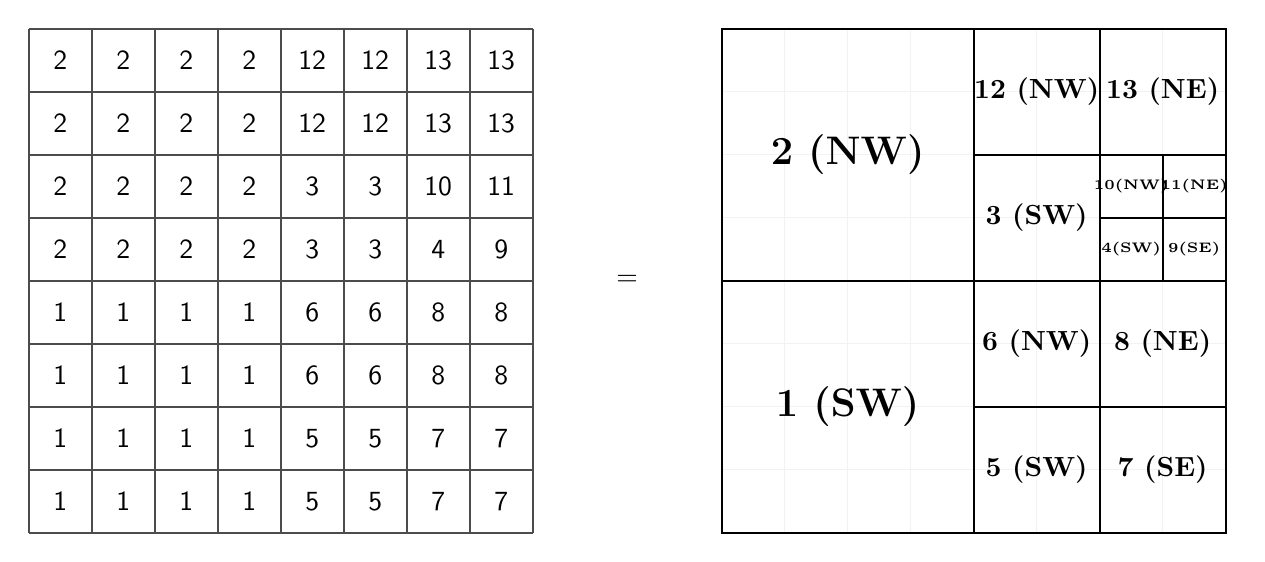
\begin{tikzpicture}[scale=0.8, font=\sffamily]

  \draw[step=1cm, black!70, thick] (0,0) grid (8,8);
  
  \foreach \x/\y/\val in {
    0/0/1, 1/0/1, 2/0/1, 3/0/1, 4/0/5, 5/0/5, 6/0/7, 7/0/7,
    0/1/1, 1/1/1, 2/1/1, 3/1/1, 4/1/5, 5/1/5, 6/1/7, 7/1/7,
    0/2/1, 1/2/1, 2/2/1, 3/2/1, 4/2/6, 5/2/6, 6/2/8, 7/2/8,
    0/3/1, 1/3/1, 2/3/1, 3/3/1, 4/3/6, 5/3/6, 6/3/8, 7/3/8,
    0/4/2, 1/4/2, 2/4/2, 3/4/2, 4/4/3, 5/4/3, 6/4/4, 7/4/9,
    0/5/2, 1/5/2, 2/5/2, 3/5/2, 4/5/3, 5/5/3, 6/5/10, 7/5/11,
    0/6/2, 1/6/2, 2/6/2, 3/6/2, 4/6/12, 5/6/12, 6/6/13, 7/6/13,
    0/7/2, 1/7/2, 2/7/2, 3/7/2, 4/7/12, 5/7/12, 6/7/13, 7/7/13
  } {
    \node at (\x+0.5, \y+0.5) {\val};
  }

\node at (9.5, 4) {$=$};

\begin{scope}[shift={(11,0)}]
    \draw[step=1cm, gray!10, very thin] (0,0) grid (8,8);
    
    \draw[draw=black, thick] (0,4) rectangle ++(4,4) node[midway, font=\Large\bfseries] {2 (NW)};
    \draw[draw=black, thick] (0,0) rectangle ++(4,4) node[midway, font=\Large\bfseries] {1 (SW)};
    
    \draw[draw=black, thick] (4,6) rectangle ++(2,2) node[midway, font=\bfseries] {12 (NW)};
    \draw[draw=black, thick] (6,6) rectangle ++(2,2) node[midway, font=\bfseries] {13 (NE)};
    \draw[draw=black, thick] (4,4) rectangle ++(2,2) node[midway, font=\bfseries] {3 (SW)};
    
    \draw[draw=black, thick] (6,4) rectangle ++(1,1) node[midway, font=\tiny\bfseries] {4(SW)};
    \draw[draw=black, thick] (7,4) rectangle ++(1,1) node[midway, font=\tiny\bfseries] {9(SE)};
    \draw[draw=black, thick] (6,5) rectangle ++(1,1) node[midway, font=\tiny\bfseries] {10(NW)};
    \draw[draw=black, thick] (7,5) rectangle ++(1,1) node[midway, font=\tiny\bfseries] {11(NE)};
    
    \draw[draw=black, thick] (4,2) rectangle ++(2,2) node[midway, font=\bfseries] {6 (NW)};
    \draw[draw=black, thick] (6,2) rectangle ++(2,2) node[midway, font=\bfseries] {8 (NE)};
    \draw[draw=black, thick] (4,0) rectangle ++(2,2) node[midway, font=\bfseries] {5 (SW)};
    \draw[draw=black, thick] (6,0) rectangle ++(2,2) node[midway, font=\bfseries] {7 (SE)};
    

  \end{scope}
\end{tikzpicture}

\label{fig:quadtree_blocks}
\end{subfigure}

\vspace{1cm}

\begin{subfigure}[b]{0.9\textwidth}
    \centering
    \caption{Quadtree representation of the blocks in~\ref{fig:quadtree_blocks}}
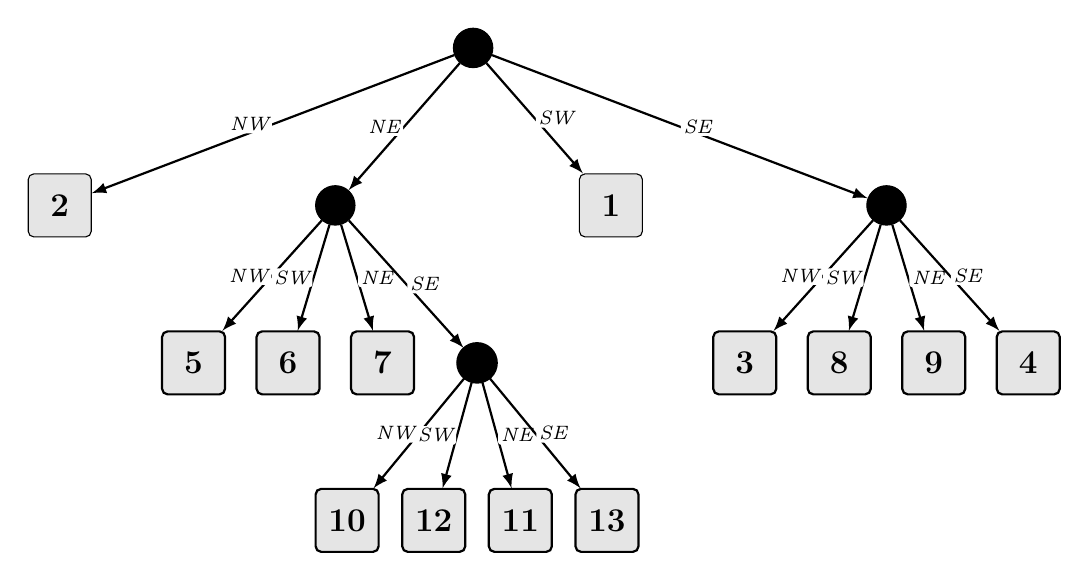
\begin{tikzpicture}[
    grow=down,
    level 1/.style={sibling distance=3.5cm, level distance=2cm},
    level 2/.style={sibling distance=1.2cm, level distance=2cm},
    level 3/.style={sibling distance=1.1cm, level distance=2cm},
    edge from parent/.style={draw, -latex, thick},
    int/.style={draw, circle, fill=black, font=\small\bfseries, minimum size=0.5cm, inner sep=0pt},
    leaf/.style={draw, rectangle, fill=gray!20, font=\large\bfseries, minimum size=0.8cm, inner sep=2pt, rounded corners=2pt},
    q/.style={font=\scriptsize\itshape, pos=0.5, fill=white, inner sep=1pt, rounded corners=1pt}
]

\node[int] { }
    child { node[leaf] {2} edge from parent node[q, left] {NW} }
    child {
        node[int] { }
        child { node[leaf] {5} edge from parent node[q, left] {NW} }
        child { node[leaf] {6} edge from parent node[q, left] {SW} }
        child { node[leaf] {7} edge from parent node[q, right] {NE} }
        child {
            node[int] {}
            child { node[leaf] {10} edge from parent node[q, left] {NW} }
            child { node[leaf] {12} edge from parent node[q, left] {SW} }
            child { node[leaf] {11} edge from parent node[q, right] {NE} }
            child { node[leaf] {13} edge from parent node[q, right] {SE} }
            edge from parent node[q, right] {SE}
            }
        edge from parent node[q, left] {NE}
    }
    child { node[leaf] {1} edge from parent node[q, right] {SW} }
    child {
        node[int] { }
        child { node[leaf] {3} edge from parent node[q, left] {NW} }
        child { node[leaf] {8} edge from parent node[q, left] {SW} }
        child { node[leaf] {9} edge from parent node[q, right] {NE} }
        child { node[leaf] {4} edge from parent node[q, right] {SE} }
        edge from parent node[q, right] {SE}
    };
\end{tikzpicture}
\label{fig:quadtree_tree}
\end{subfigure}
\label{fig:quadtree_example}
\end{figure}



This recursive partitioning allows large uniform blocks to be represented implicitly, eliminating the need to store them explicitly.
Unlike flat array formats such as CSR or CSC, which are standard in libraries like SuiteSparse:GraphBLAS, the quad-tree naturally supports a divide-and-conquer execution model and adapts dynamically to irregular sparsity patterns.
This structure simplifies parallelization, as independent sub-blocks can be processed recursively without global synchronization.

However, this flexibility comes at a cost: for dense or highly regular matrices, the overhead of maintaining tree metadata and pointer indirection can outweigh the benefits of sparse storage, making traditional linear formats more efficient in such cases.


\subsection{Interaction Nets}

\label{sec:interaction_nets}

We utilize the variant of definitions provided by Y. Lafont in 1989~\cite{10.1145/96709.96718}. Interaction Nets is a graph-rewriting model where computation proceeds through local rewriting rules applied to pairs of connected nodes.

\textit{(Agent)}. An \textit{agent} is a symbol from a fixed alphabet $\Sigma$, for which:
\begin{itemize}
    \item an arity is defined --- a function $Ar: \Sigma \to \mathbb{N} \cup \{0\}$;
    \item there is one \textit{principal port} and a number of \textit{auxiliary ports} equal to its arity.
\end{itemize}

\textit{(Net)}. A \textit{net} over the alphabet $\Sigma$ is a labeled undirected multi-graph in which:
\begin{itemize}
    \item each node is labeled by an agent;
    \item edges can only exist between ports;
    \item at most one edge enters each port.
\end{itemize}

Let $\mathcal{N}_\Sigma$ denote the set of all possible nets over the alphabet $\Sigma$.

We say that a port is \textit{free} if no edge originates from it. A net can also consist simply of a set of edges, in which case each end of an edge is considered a free port.

\textit{(Interface)}. The \textit{interface} $I(n)$ is the set of all free ports of a net $n$.

We say that port $p_a$ is connected to port $p_b$ if there is an edge between them.
An example of a simple net is shown in figure~\ref{fig:in_example}.
The set of agents is $\Sigma=\{\beta, \alpha\}$ with arities $Ar(\beta)=0$, $Ar(\alpha)=2$.
The principal ports of the $\alpha$-nodes are connected to each other, and the principal port of the $\beta$-node is connected to one of the auxiliary ports of the left $\alpha$-node.
There are three free ports: one at the left $\alpha$-agent and two at the right $\alpha$-agent.
These constitute the interface.

\begin{figure}[h]
    \centering
    \caption{Example of a net consisting of three nodes}
    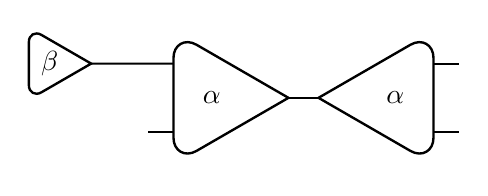
\begin{tikzpicture}
        \matrix[column sep = 1em]{
            \inetcell(b) {$\phantom x\alpha\phantom x$}[R] &
            \inetcell(a) {$\phantom x\alpha\phantom x$}[L]   \\
        };
        \inetcell[left = of b.left pax, distance=1em](out) {$\beta$}[R]
        \inetwirefree(a.left pax)
        \inetwirefree(a.right pax)
        \inetwire(a.pal)(b.pal)
        \inetwire(b.left pax)(out.pal)
        \inetwirefree(b.right pax)
    \end{tikzpicture}
    \label{fig:in_example}
\end{figure}


Computation in Interaction Nets occurs via \textit{reductions}: rewriting an \textit{active pair} into a net. An active pair is defined as two agents connected via their principal ports.

\textit{(Reduction Rule)}. A \textit{reduction rule} is a graph rewriting rule. Let $R$ be the set of reduction rules. More formally, a reduction rule is a triplet $r \in \Sigma \times \Sigma \times \mathcal{N}_\Sigma$, for which the following properties hold:
\begin{itemize}
    \item \textbf{Symmetry:} $(l_1, l_2, n) \in R \Rightarrow (l_2, l_1, n) \in R$
    \item \textbf{Determinism:} $(l_1, l_2, n_1) \in R \land (m_1, m_2, n_2) \in R \Rightarrow (l_1, l_2) \neq (m_1, m_2)$
    \item \textbf{Interface Preservation:} $\forall (l_1, l_2, n) \in R, Ar(l_1) + Ar(l_2) = \|I(n)\|$
\end{itemize}


As shown in Lafont's work~\cite{10.1145/96709.96718}, $\lambda$-calculus can be expressed through this formalism. Additionally, reductions can be performed independently of each other and it has been proven that the order of reductions doesn't matter. This serves as the primary reason for the natural suitability of Interaction Nets for parallel computations.

\subsection{Inpla}

Introduce Inpla: runtime (VM) and language.
Briefly describe its syntax for defining agents and rules, and how it allows to program these graph-rewriting systems.
This section sets the stage for understanding our Inpla-based implementation.

\subsection{Vine}

IVY, IVM. Differences with Inpla.
\section{Implementation Details}\label{sec:API}

\subsection{Implemented Basic Functions}\label{sec:graph_algorithms}

Algebraic data types.

Options.

Structures not only for power of 2.

\begin{listing}
\begin{minted}{ocaml}
    type treeValue<'value> =
       | Dummy
       | UserValue of 'value
\end{minted}
\caption{!!!}
\end{listing}

\begin{listing}
\begin{minted}{ocaml}
(*
| x1 | x2 |
----------
| x3 | x4 |
*)
type qtree<'value> =
    | Node of qtree<'value> * qtree<'value> * qtree<'value> * qtree<'value>
    | Leaf of treeValue<'value>

[<Struct>]
type Storage<'value> =
    // Storage is always size-x-size square.
    val size: uint64<storageSize>
    val data: qtree<'value>

    new(_size, _data) = { size = _size; data = _data }

[<Struct>]
type SparseMatrix<'value> =
    val nrows: uint64<nrows>
    val ncols: uint64<ncols>
    val nvals: uint64<nvals>
    val storage: Storage<Option<'value>>

\end{minted}
\caption{!!!}
\end{listing}

List of functions: map, mpa2, mask as map2, vxm, mxm. Conversion form-to coordinate list.

Exceptions handling?

\subsection{Implemented Graph Analysis Algorithms}\label{sec:graph_algorithms}

implemented algorithms: level-bfs BFS, SSSP with control , Triangles counting (name?).

\subsection{Interaction Nets Related Details}

Translation almost ``as-is'' but...

Fixes in Inpla: list reading, !!!!

Inpla has no IO, so generated data structures.

Vine? With reading. In parallel, so hard to separate.

\section{Evaluation}\label{sec:evaluation}

The goal of this evaluation is to assess the applicability of runtimes based on Interaction Nets to real-world problems, identify bottlenecks and issues, and highlight directions for further investigation.

\subsection{Experimental Setup}

\paragraph{Hardware.}
All experiments were conducted on a system with an AMD Ryzen 7 5800X 8-core processor (16 threads with hyper-threading enabled, base clock 3.8 GHz) and 128 GiB of DDR5 RAM.

\paragraph{Software.}
We compare five implementations presented below.
\begin{itemize}
    \item \textbf{F\#}: Our quadtree-based single-threaded implementation\footnote{Quad-tree-based linear algebra in F\#: \url{https://github.com/Lamagraph/QTreeFSharp}.} that written in F\# and compiled for the .NET 10.0 runtime.
    This serves as a baseline representing a conventional functional language approach and prototype for porting to Interaction Nets.
    We use BenchmarkDotNet\footnote{BenchmarkDotNet project: \url{https://github.com/dotnet/BenchmarkDotNet}}\cite{Akinshin2019} for benchmarking automation (e.g., for JIT warmup).
	\item \textbf{Inpla (version 0.13.4, patched)\footnote{Patched version of Inpla: \url{https://github.com/Lamagraph/inpla}.}}: Our interaction-net-based implementation\footnote{Quad-tree-based linear algebra in Inpla: \url{https://github.com/Lamagraph/QTreeInpla}.} in Inpla low-level language, executed on the Inpla runtime system.
	Our patches of Inpla allow one to use arbitrary heap size configuration with per-thread adjustments via scripting.
    The patch also increases several virtual machine compile-time constants to support very large trees (thus, large graphs).
    Additionally, a bottleneck in lists parsing was discovered during testing, and the fix has since been merged into the main Inpla repository\footnote{Change request to Inpla with lists paring fix: \url{https://github.com/inpla/inpla/pull/4}}.
    Three or five runs for each configuration depending on data size.
    \item \textbf{Vine (commit \#41e5ec67)\footnote{Installed using instructions from \href{https://vine.dev/docs/starting/installation}{documentation}.}}: Our interaction-net-based implementation\footnote{Quad-tree-based linear algebra in Vine: \url{https://github.com/Lamagraph/QTreeVine}.} in Vine high-level language, executed on the Vine runtime system. We set 110 GB of heap per worker. Five runs for each configuration
    \item \textbf{LAGraph (version 1.2.1)}: A collection of graph algorithms built on SuiteSparse:GraphBLAS (version 10.3.1), providing state-of-the-art, linear-algebra-based reference implementations of BFS, SSSP, and triangle counting. 
    We use the provided algorithms as a SOTA baseline for high-performance parallel graph analysis. 
    Additionally, we use LAGraph as a baseline to analyze scaling across available threads. 
    We perform 10 runs for each configuration.
    \item \textbf{NetworkX (version 3.6.1)}: A popular Python library for graph analysis.
    We use the algorithms implemented in NetworkX as a well-known baseline.
    We do not use any special backends for NetworkX or special settings.
    We perform 10 runs for each configuration.
\end{itemize}

\begin{wraptable}{r}{7cm}
\centering
\caption{Dataset properties}
\label{tab:datasets}
\begin{tabular}{l r r}
\hline
Graph & \(|V|\) & \(|E|\) \\
\hline
coAuthorsCiteseer & 227,320 & 1,628,268  \\
boneS01 & 127,224 & 5,516,602  \\
usroads-48 & 126,146 & 323,900 \\
Andrews & 60,000 & 760,154 \\
Trefethen\_2000 & 2000 & 41,906 \\
gr\_30\_30 & 900 & 7,744 \\
\hline
\end{tabular}
\end{wraptable}
\paragraph{Dataset.}
We evaluate our implementations on several real-world and synthetic graphs from the SuiteSparse Matrix Collection~\cite{Kolodziej2019}.
The graphs are chosen to represent a variety of sizes, sparsity patterns, and application domains, taking into account the capabilities and limitations of the selected competitors.
Table~\ref{tab:datasets} summarizes the number of vertices (\(|V|\)) and edges (\(|E|\)) of the selected graphs.
Weights were shifted relative to the minimum weight per graph to prevent negative cycles and were converted to \texttt{Int} because Inpla does not support floats.
All graphs were converted to undirected and have exactly one connected component; thus, any vertex can be selected as a start for BFS and SSSP. 
We selected Vertex 0 for all runs.

\paragraph{Reordering.} Sparse matrix reordering techniques can improve performance of operations over matrices~\cite{10.1145/3731599.3767441}.
In case of quad-tree based represenation reordering also can reduce memory consumption.
We use reverse Cuthill--McKee for reordering.
Patterns for selected matrices is represented in Figure~\ref{fig:matrices_patterns}. 
Patterns for \emph{gr\_30\_30} is similar to patterns for \emph{boneS01}. 
In evaluation we use both original and reordered matricses except \emph{coAuthorsCiteseer} that used reordered only version because original version cause OOM of Inpla.
We can see, that in this case reordered matrix has big empty blocks that represented in qud-tree compactly.
Similarly for \emph{Andrews}. For other matrices reordering effect was investigated in evaluation.

\begin{figure*}[t!]
    \centering
    \begin{subfigure}[t]{0.195\textwidth}
        \centering
        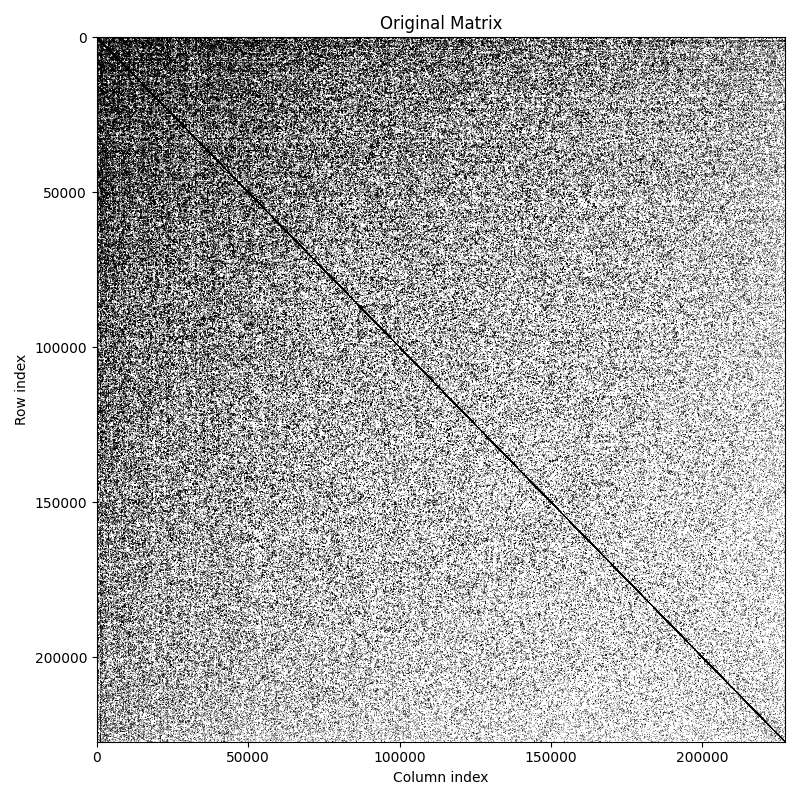
\includegraphics[width=\textwidth]{figures/original_coAuthors.png}
        \caption{coAuthorsCiteseer}
    \end{subfigure}
    \begin{subfigure}[t]{0.195\textwidth}
        \centering
        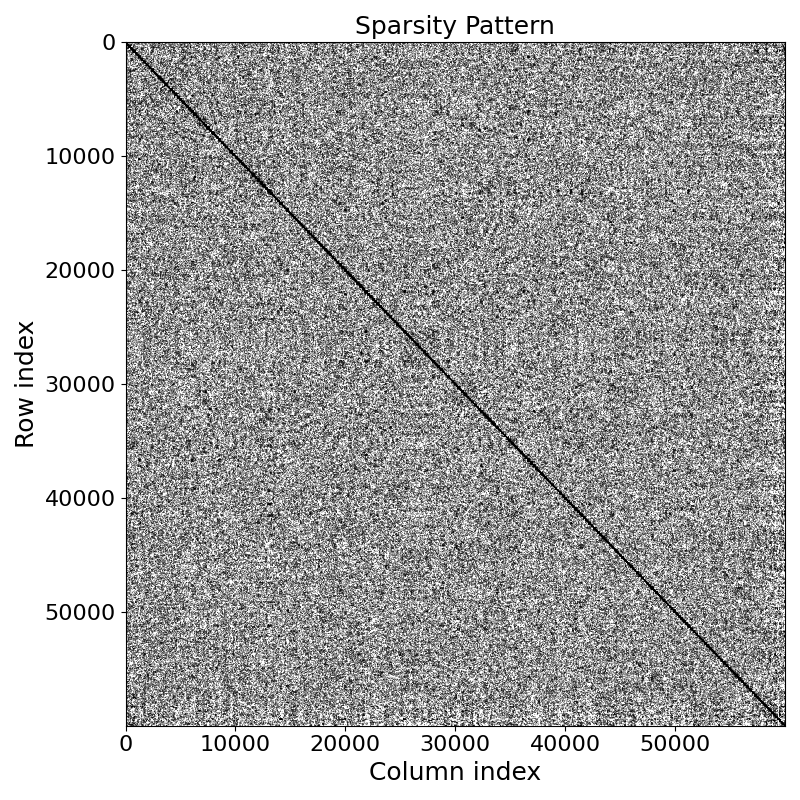
\includegraphics[width=\textwidth]{figures/original_Andrews_positive.png}
        \caption{Andrews}
    \end{subfigure}
    \begin{subfigure}[t]{0.195\textwidth}
        \centering
        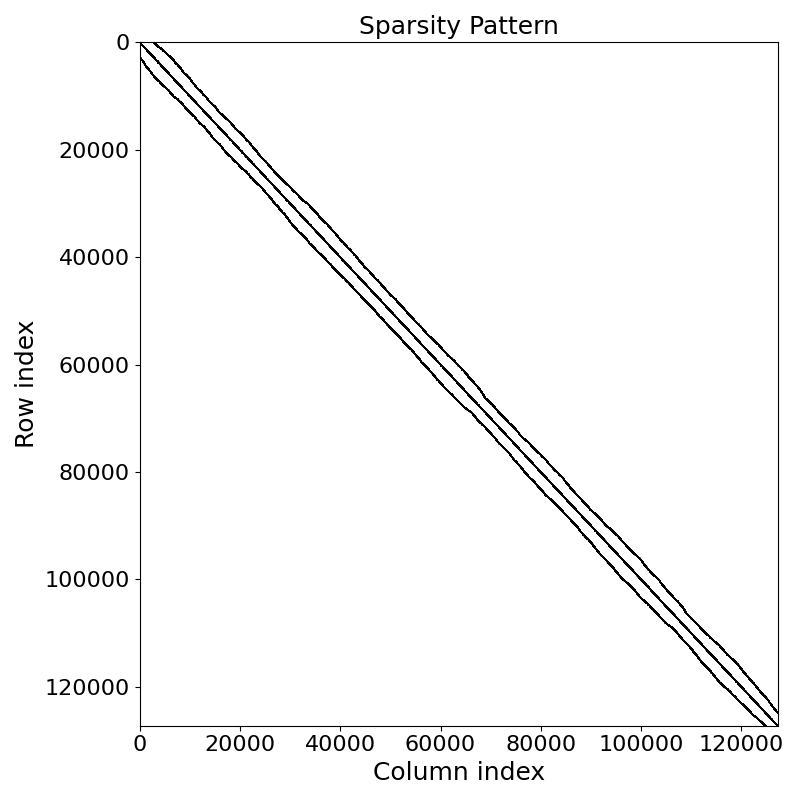
\includegraphics[width=\textwidth]{figures/original_boneS01.png}
        \caption{boneS01}
    \end{subfigure}
    \begin{subfigure}[t]{0.195\textwidth}
        \centering
        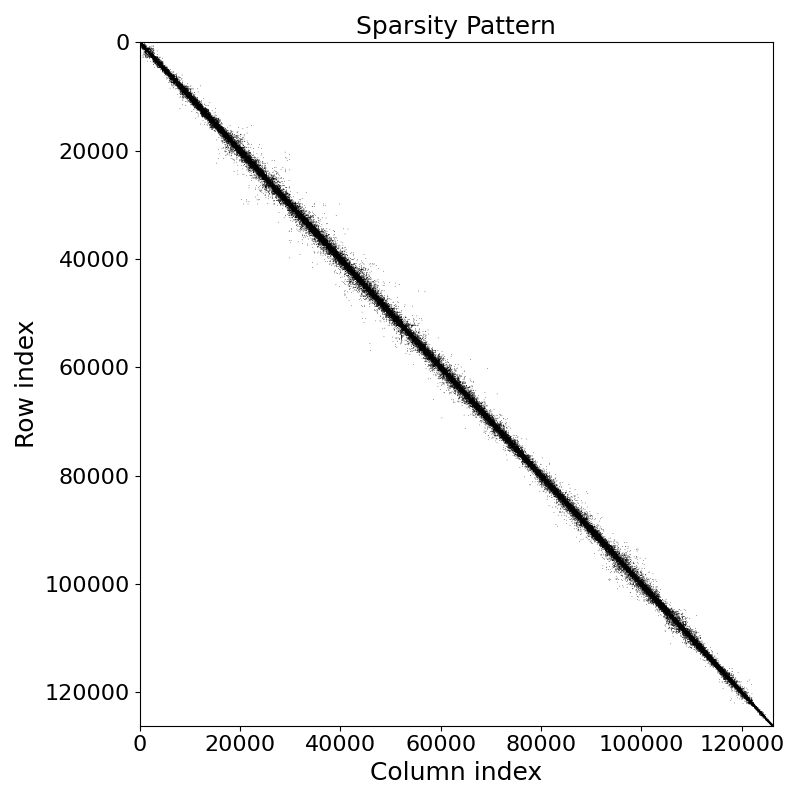
\includegraphics[width=\textwidth]{figures/original_usroads_48.png}
        \caption{usroads-48}
    \end{subfigure}
    \begin{subfigure}[t]{0.195\textwidth}
        \centering
        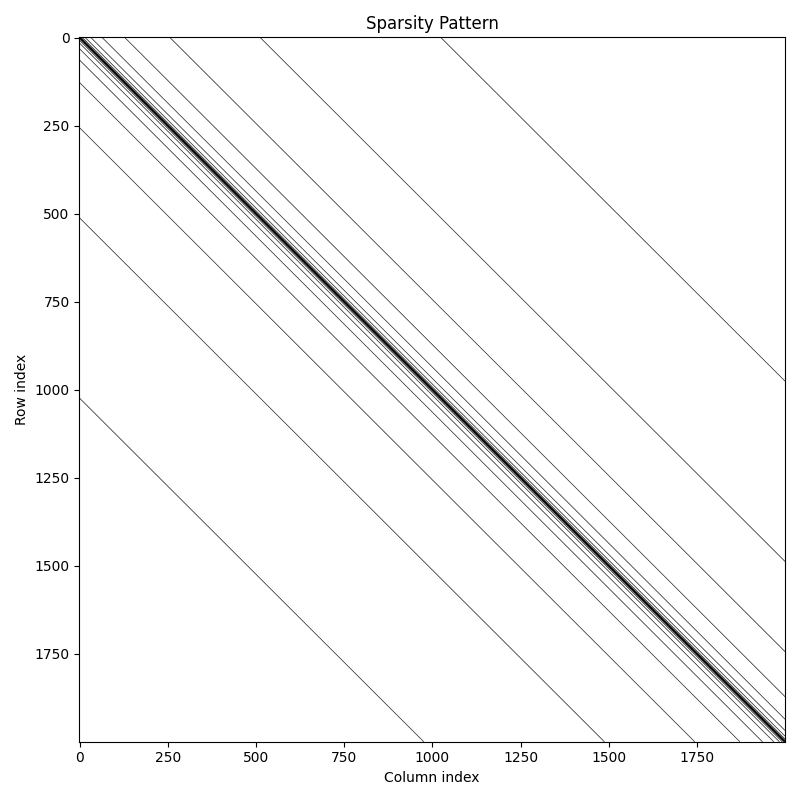
\includegraphics[width=\textwidth]{figures/original_Trefethen_2000.png}
        \caption{Treferthen\_2000}
    \end{subfigure}%
 
    \begin{subfigure}[t]{0.195\textwidth}
        \centering
        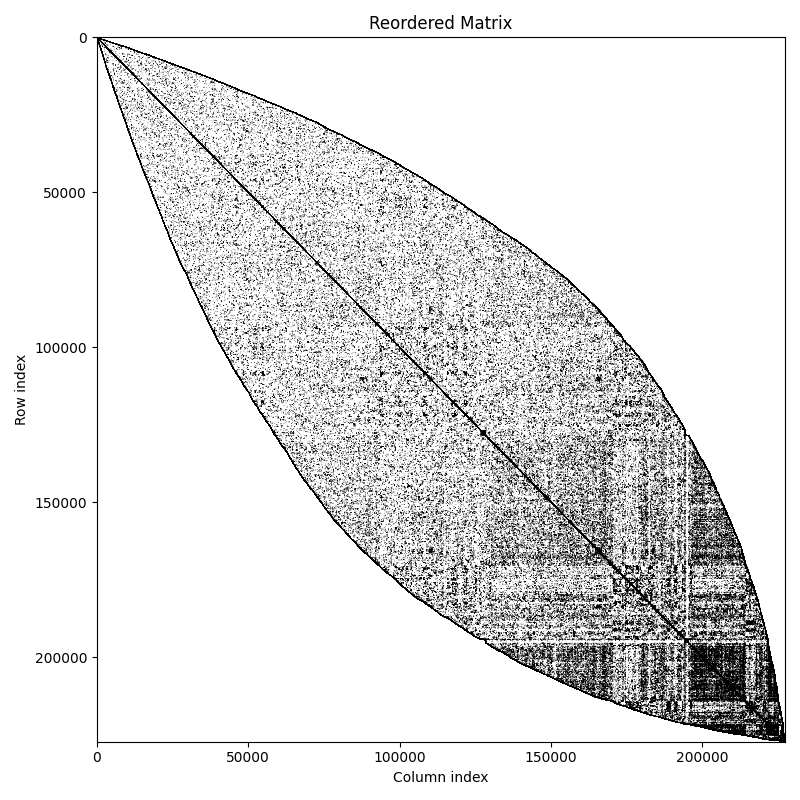
\includegraphics[width=\textwidth]{figures/reordered_coAuthors.png}
        \caption{coAuthorsCieseer}
    \end{subfigure}
    \begin{subfigure}[t]{0.195\textwidth}
        \centering
        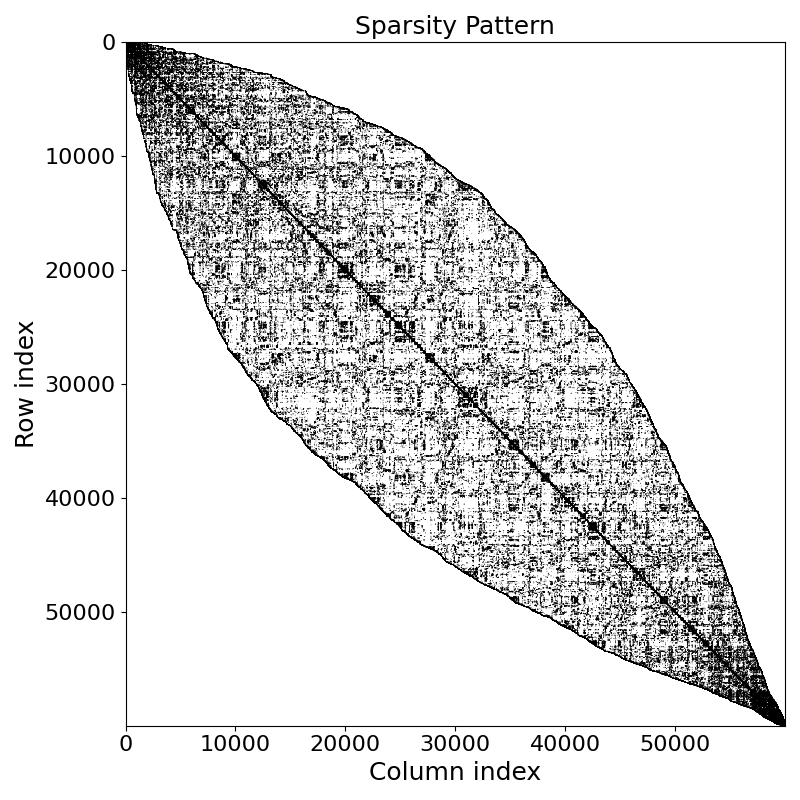
\includegraphics[width=\textwidth]{figures/reordered_Andrews_positive.png}
        \caption{Andrews}
    \end{subfigure}
    \begin{subfigure}[t]{0.195\textwidth}
        \centering
        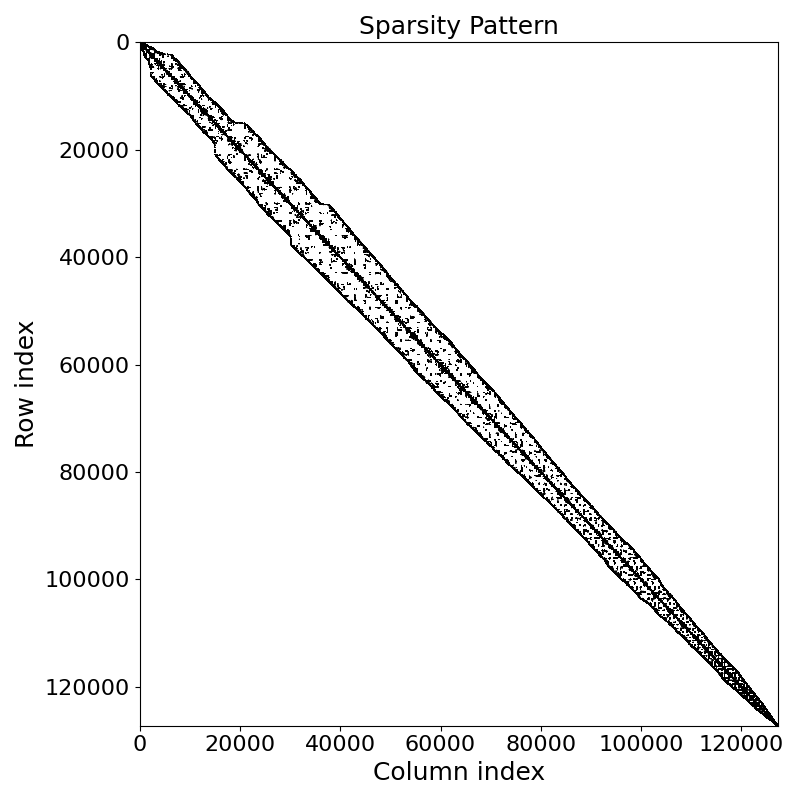
\includegraphics[width=\textwidth]{figures/reordered_boneS01.png}
        \caption{boneS01}
    \end{subfigure}
    \begin{subfigure}[t]{0.195\textwidth}
        \centering
        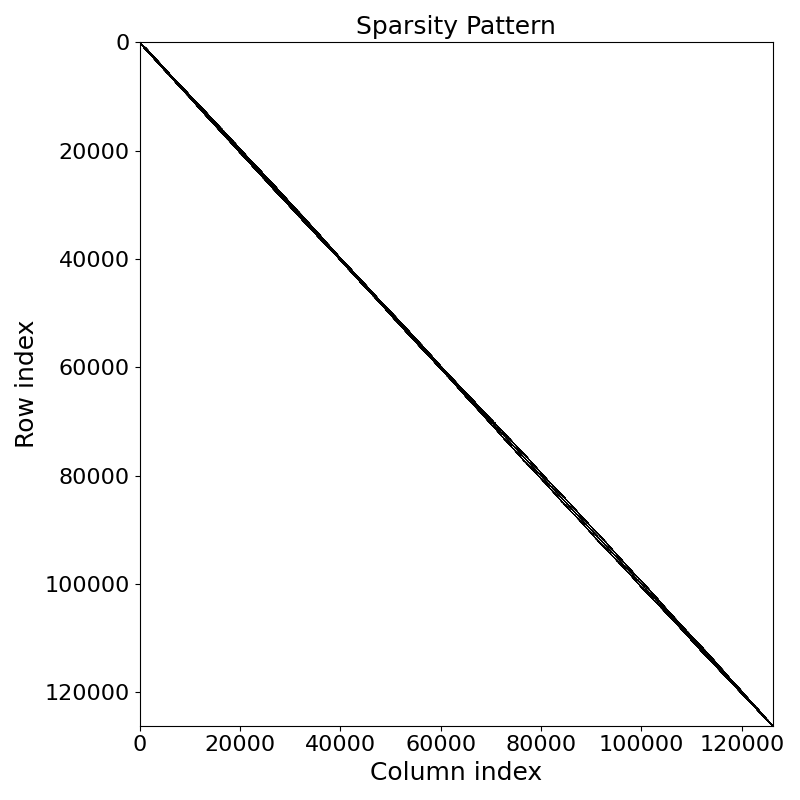
\includegraphics[width=\textwidth]{figures/reordered_usroads_48.png}
        \caption{usroads-48}
    \end{subfigure}
    \begin{subfigure}[t]{0.195\textwidth}
        \centering
        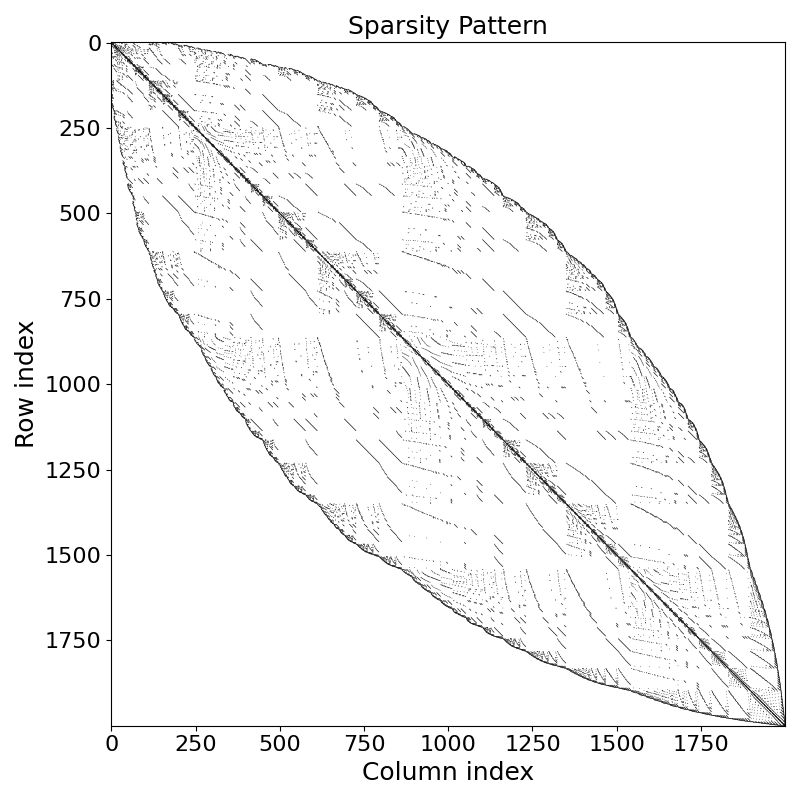
\includegraphics[width=\textwidth]{figures/reordered_Trefethen_2000.png}
        \caption{Treferthen\_2000}
    \end{subfigure}
    \caption{Matrices shapes: original and after reordering}
    \label{fig:matrices_patterns}
\end{figure*}

\begin{figure*}[t!]
    \centering
    \begin{subfigure}[t]{0.33\textwidth}
        \centering
        \includegraphics[width=\textwidth]{figures/bfs_coAuthorsCiteseer_reordered.pdf}
        \caption{Execution time}
        \label{fig:coAuthors_execution_time}
    \end{subfigure}
    ~
    \begin{subfigure}[t]{0.33\textwidth}
        \centering
        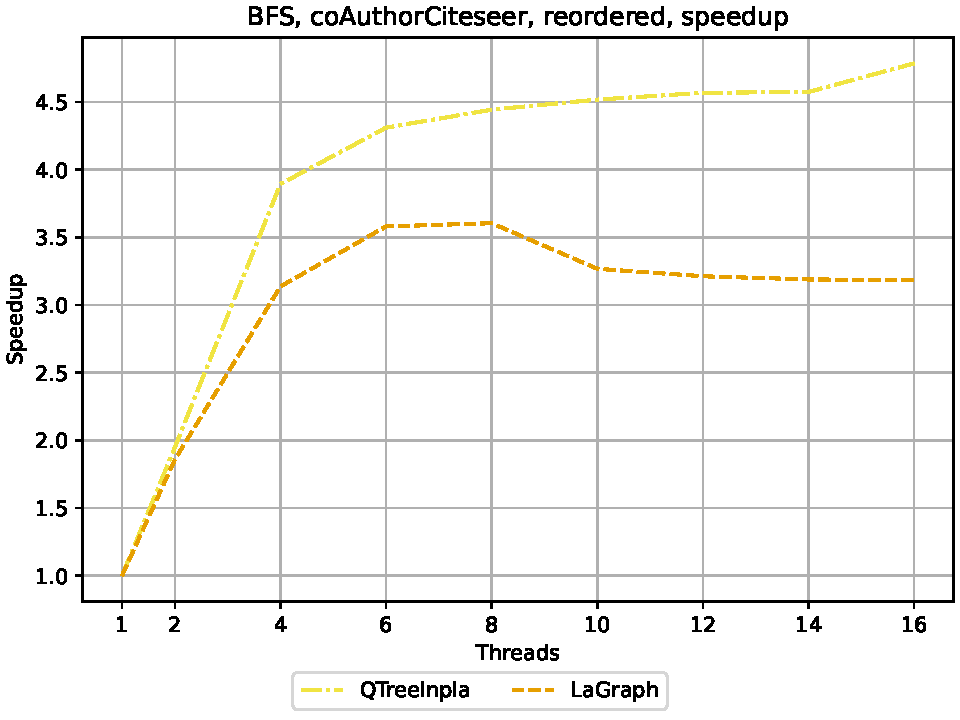
\includegraphics[width=\textwidth]{figures/bfs_coAuthorsCiteseer_reordered_speedup.pdf}
        \caption{Scaling}
        \label{fig:coAuthors_scaling}
    \end{subfigure}
    \caption{Evaluation results for BFS on \emph{coAuthorsCiteseer} (reordered)}
\end{figure*}

\begin{figure*}[t!]
    \centering
    \begin{subfigure}[t]{0.33\textwidth}
        \centering
        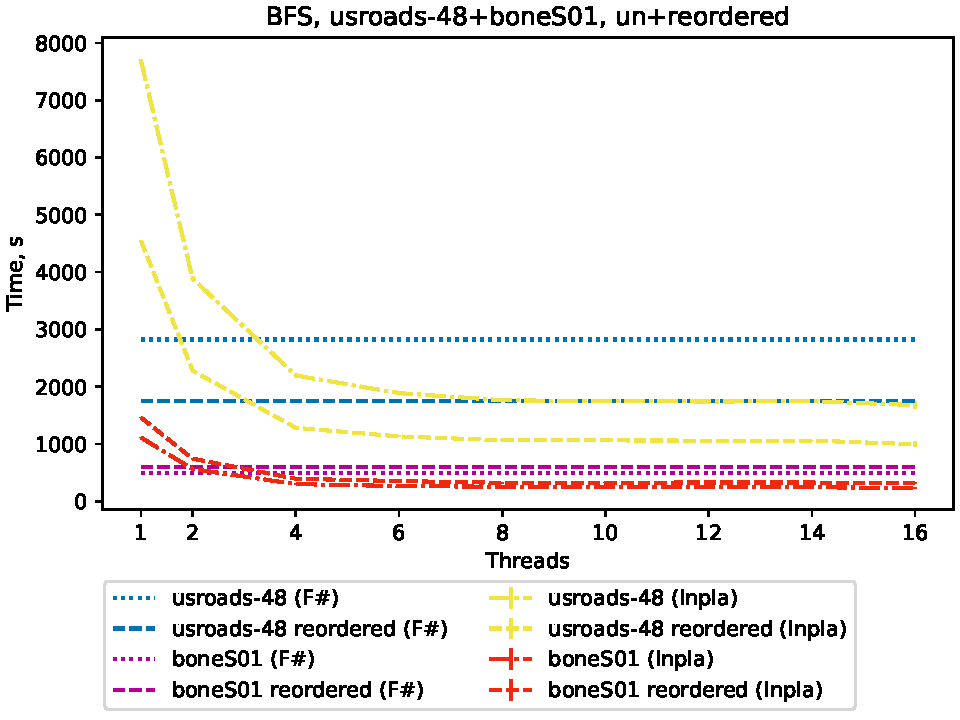
\includegraphics[width=\textwidth]{figures/usroads_and_bone_all.pdf}
        \caption{Execution time}
        \label{fig:bone_and_usroads_execution_time}
    \end{subfigure}
    ~
    \begin{subfigure}[t]{0.33\textwidth}
        \centering
        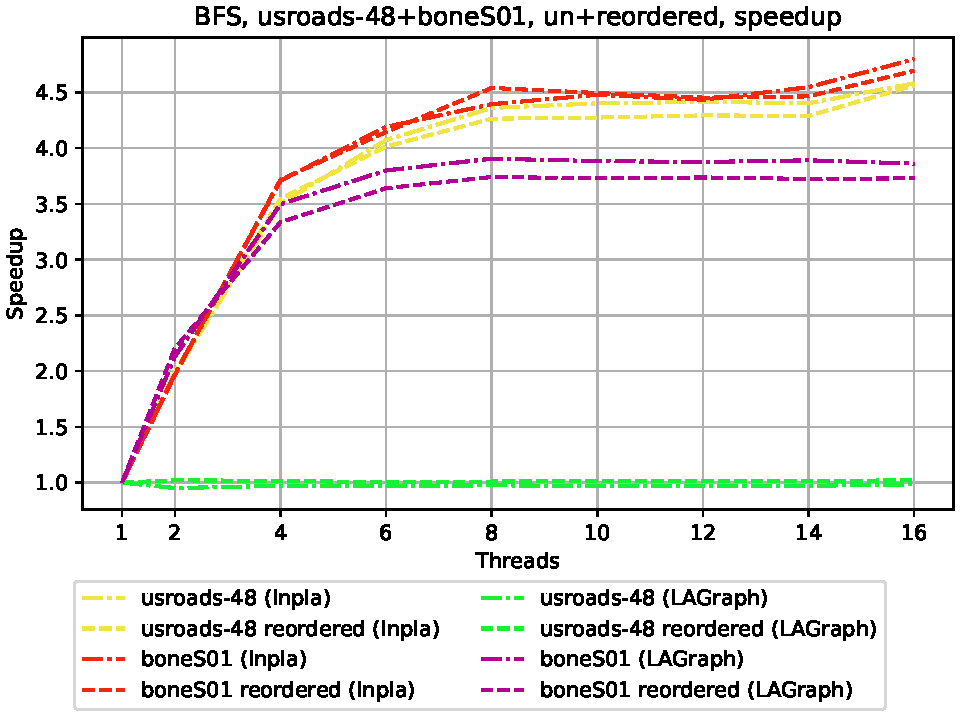
\includegraphics[width=\textwidth]{figures/usroads_and_bone_all_speedup.pdf}
        \caption{Scaling}
        \label{fig:bone_and_usroads_scaling}
    \end{subfigure}
    \caption{Evaluation results for BFS on \emph{bomeS01} and \emph{usroads-48} (both original and reordered)}
\end{figure*}

\begin{figure*}[t!]
    \centering
    \begin{subfigure}[t]{0.33\textwidth}
        \centering
        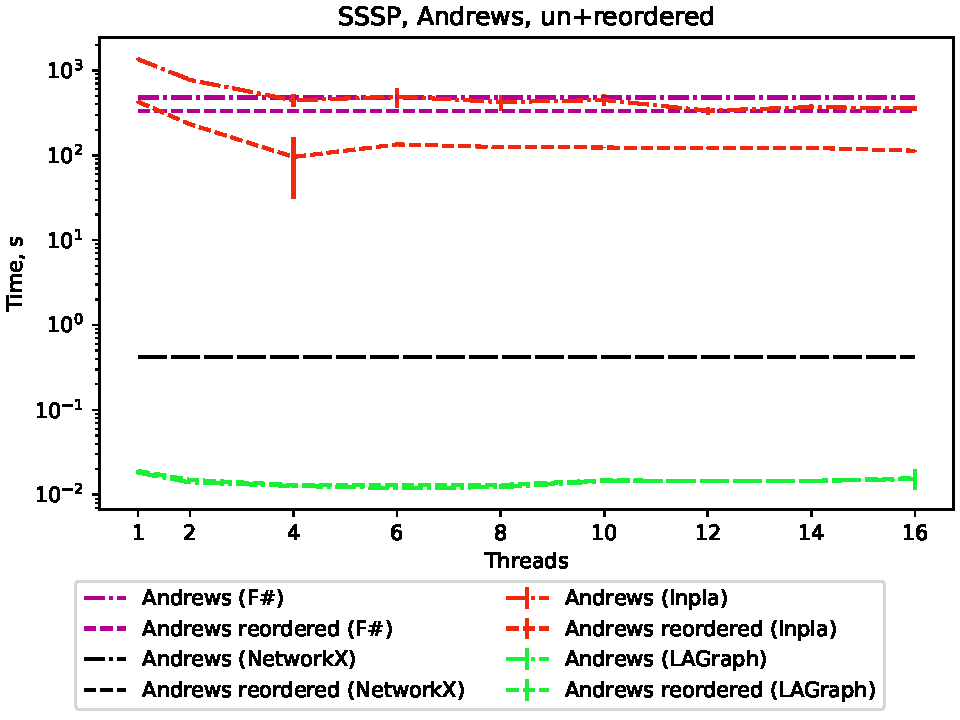
\includegraphics[width=\textwidth]{figures/sssp_andrews_positive.pdf}
        \caption{Execution time}
        \label{fig:andrews_execution_time}
    \end{subfigure}
    ~
    \begin{subfigure}[t]{0.33\textwidth}
        \centering
        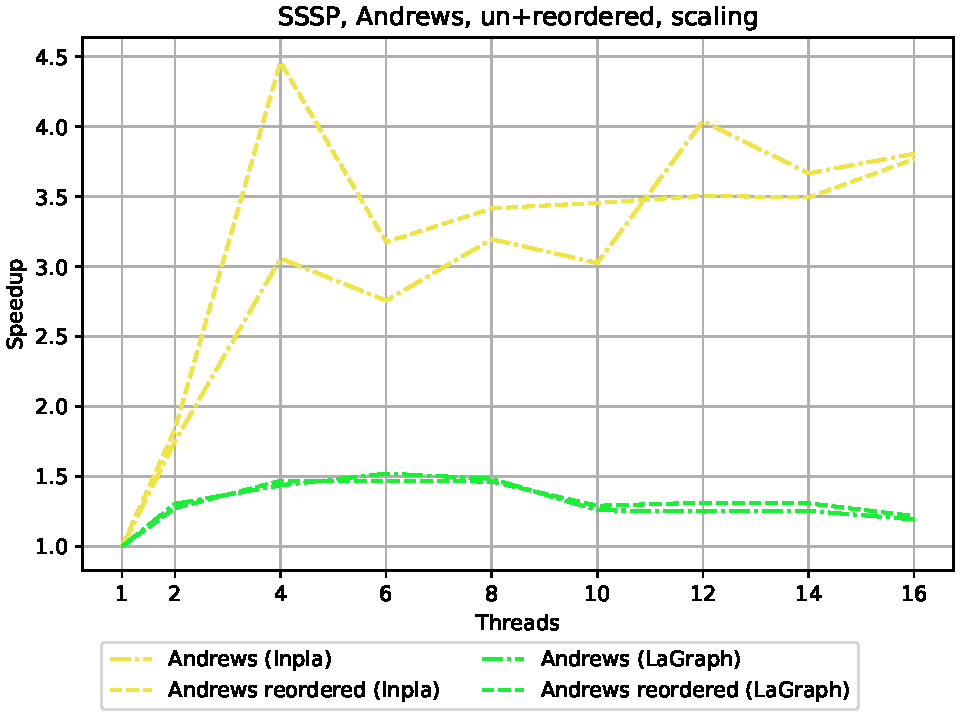
\includegraphics[width=\textwidth]{figures/sssp_andrews_positive_scaling.pdf}
        \caption{Scaling}
        \label{fig:andrews_scaling}
    \end{subfigure}
    \caption{SSSP evaluation results for \emph{Andrews} (both original and reordered)}
\end{figure*}

\begin{figure*}[t!]
    \centering
    \begin{subfigure}[t]{0.32\textwidth}
        \centering
        \includegraphics[width=\textwidth]{figures/bfs_treferthen_2000.pdf}
        \caption{BFS}
        \label{fig:bfs_treferthen_execution_time}
    \end{subfigure}
    ~
    \begin{subfigure}[t]{0.32\textwidth}
        \centering
        \includegraphics[width=\textwidth]{figures/sssp_treferthen_2000.pdf}
        \caption{SSSP}
        \label{fig:sssp_treferthen_execution_time}
    \end{subfigure}
    ~
    \begin{subfigure}[t]{0.32\textwidth}
        \centering
        \includegraphics[width=\textwidth]{figures/treferthen_2000_sssp_speedup.pdf}
        \caption{SSSP scaling}
        \label{fig:bfs_treferthen_scaling}
    \end{subfigure}
    \caption{Evaluation results for \emph{Treferthen\_2000} (both original and reordered)}
    
\end{figure*}


\begin{figure*}[t!]
    \centering
    \begin{subfigure}[t]{0.32\textwidth}
        \centering
        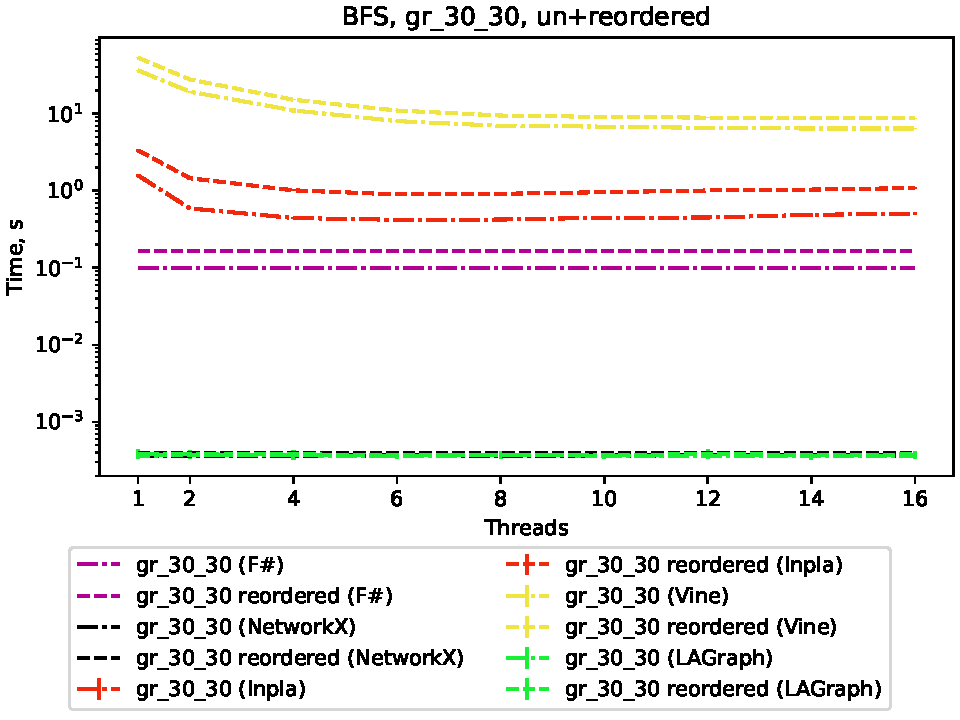
\includegraphics[width=\textwidth]{figures/bfs_gr_30_30.pdf}
        \caption{BFS}
        \label{fig:bfs_gr_3_30_execution_time}
    \end{subfigure}
    ~
    \begin{subfigure}[t]{0.32\textwidth}
        \centering
        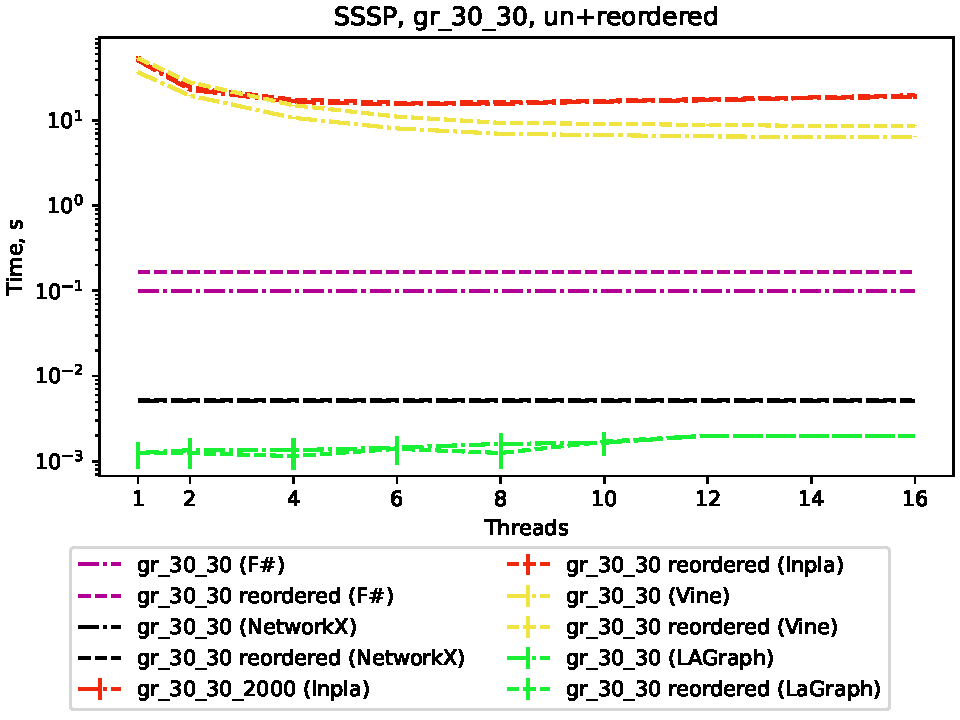
\includegraphics[width=\textwidth]{figures/sssp_gr_30_30.pdf}
        \caption{SSSP}
        \label{fig:sssp_gr_3_30_execution_time}
    \end{subfigure}
    ~
    \begin{subfigure}[t]{0.32\textwidth}
        \centering
        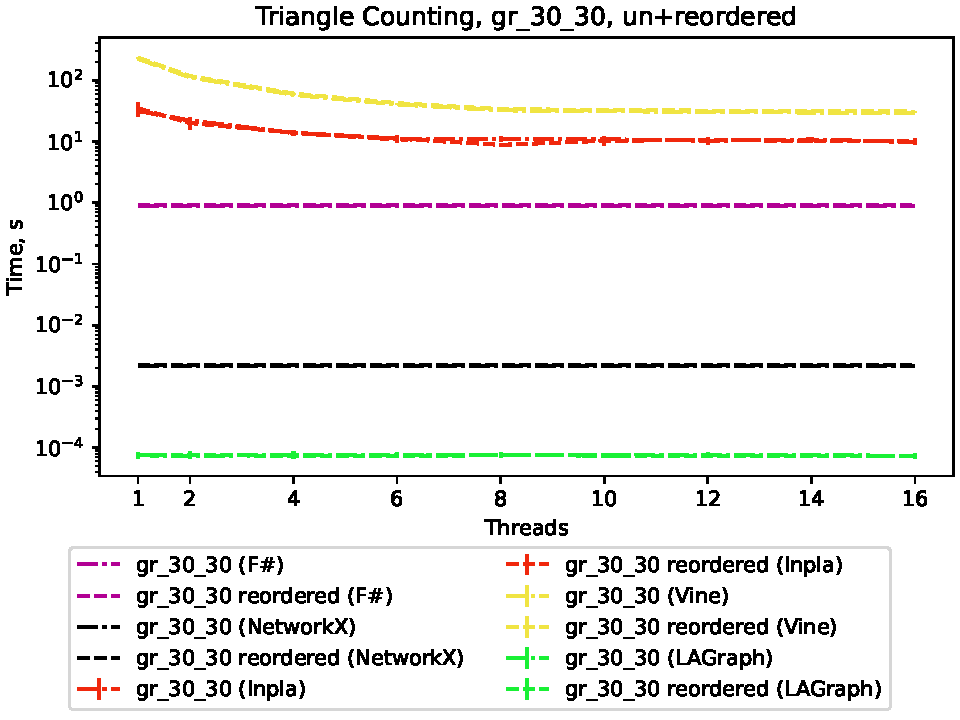
\includegraphics[width=\textwidth]{figures/tc_gr_30_30.pdf}
        \caption{Triangle counting}
        \label{fig:tc_gr_3_30_execution_time}
    \end{subfigure}
    \caption{Evaluation results for \emph{gr\_30\_30} (both original and reordered)}
    
\end{figure*}

\begin{figure*}
    \centering
    \begin{subfigure}[t]{0.33\textwidth}
        \centering
        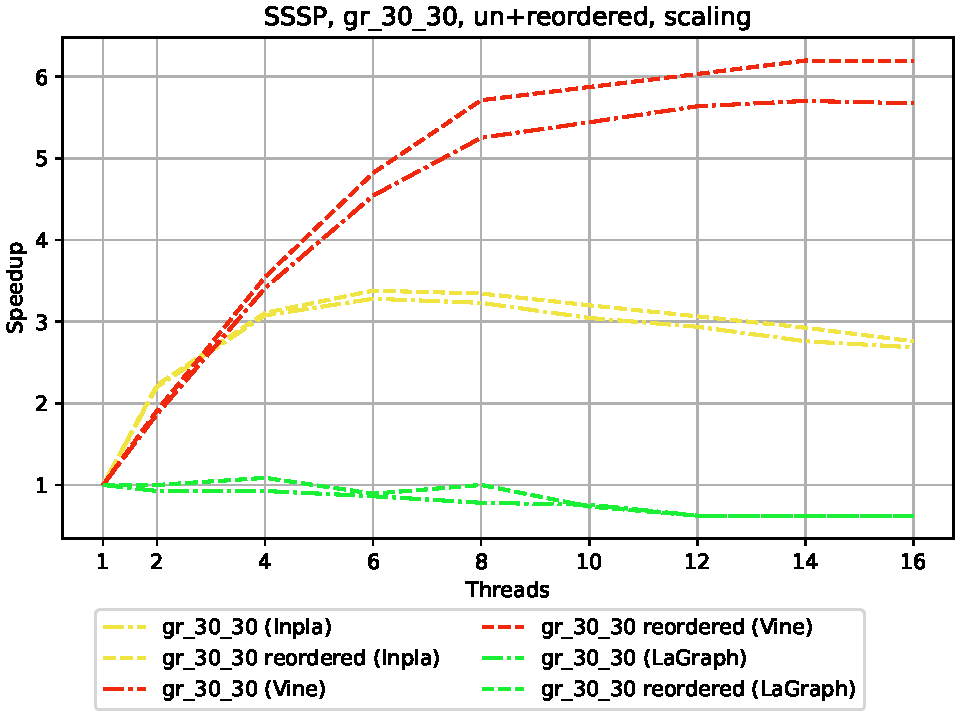
\includegraphics[width=\textwidth]{figures/sssp_gr_30_30_scaling.pdf}
        \caption{BFS scaling}
        \label{fig:bfs_gr_3_30_scaling}
    \end{subfigure}
    \begin{subfigure}[t]{0.33\textwidth}
        \centering
        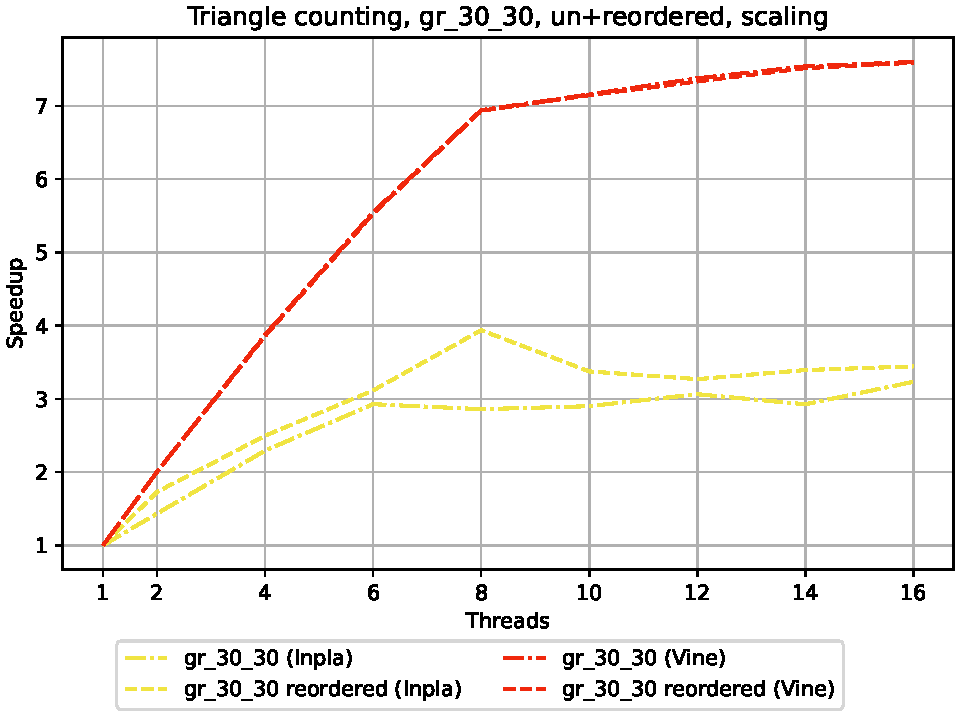
\includegraphics[width=\textwidth]{figures/tc_gr_30_30_scaling.pdf}
        \caption{Triangle counting scaling}
        \label{fig:tc_gr_3_30_scaling}
    \end{subfigure}
    \caption{!!!}
\end{figure*}

\paragraph{Research Questions.}
Our evaluation addresses the following research questions:

\begin{description}
    \item[RQ1 (Performance).] How does the execution time of Inpla an Vine compare to LAGraph, NetworkX and F\# on BFS, SSSP, and triangle counting?

    \item[RQ2 (Scaling).] How well do the Inpla, Vine, and LAGraph implementations scale with the number of available CPU cores?
          We measure speedup from 1 to all available cores for BFS, SSSP, and triangle counting.

    \item[RQ3 (Impact of Matrix Reordering).] 
          How does reordering affect the performance of competitors?
\end{description}

\subsection{Evaluation Results}

First, we discuss the limitations that prevented evaluating all (graph, algorithm, tool) combinations. 
The primary limitation is the substantial memory consumption of Inpla and Vine.
Since our implementations rely on a recursive divide-and-conquer computation pattern, aggressive duplication occurs during computations. 
While BFS and SSSP require only the \verb|vxm| operation, triangle counting requires the \verb|mxm| operation, which involves more complex recursive calls. As a result, triangle counting is feasible only on relatively small graphs. Notably, Vine encounters out-of-memory (OOM) errors even on \emph{Trefethen\_2000} when performing triangle counting.
Second, Vine is excessively slow.
Therefore, we can execute it within a reasonable time only on small matrices, namely \emph{Trefethen\_2000} and \emph{gr\_30\_30}.
Additionally, Inpla has dataraces that leads to instability\footnote{Some of them already fixed by our team (e.g. this one: \url{https://github.com/inpla/inpla/pull/8}), other must be fixed in the future.}.
We check that results are correct, but des not guarantee that raises does not affect performance patterns.

Regarding \textbf{performance} we can see, that in all cases (Figures~\ref{fig:coAuthors_execution_time},~\ref{fig:bone_and_usroads_execution_time},~\ref{fig:andrews_execution_time},~\ref{fig:bfs_treferthen_execution_time},~\ref{fig:sssp_treferthen_execution_time},~\ref{fig:bfs_gr_3_30_execution_time},~\ref{fig:sssp_gr_3_30_execution_time}) Interaction Nts based implamantations in several orders of magnitude slower (up to $10^5$) then both NetworkX and LAGraph. 
Note that in almost the all cases LAGraph is faster that NetworkX. So for all selected cases linear algebra based approach can demonstrate reasonable perforamnce.
We can conclude that if graph is big enough (\emph{coAuthorsCiteseer, boneS01, usroads-48, Andrews}) then Inpla can outperforms F\# implementation.
Note that  

Inpla slower in case SSSP on \emph{gr\_30\_30} Moreover inpla scales very bad in this case.
It may be cased by manual tuning of parameters aimed on performance on big grpahs.

\textbf{Scaling}.
Near to linear scaling on up to 4 threads.
Inpla scales better than LAGraph: 
Complex scaling pattern of LAGraph and more evident for Inpla and Vine.
Vine scale better than Inpla.
On small data (\emph{Treferthen\_2000} and \emph{gr\_30\_30}) Inpla scales poor.

\textbf{Reordering} analysis shows that in cases when initial matrix has no specific pattern (\emph{coAuthorsCiteseer} and \emph{Andrews}) it helps to reduce memory consumption and to improve performance.
In cases when matrix has diagonal-like initial pattern contribution of reordering is not so trivial. 
Inpla: For \emph{usroads-48} reordered faster. 
For \emph{boneS01} reordered is slower. Note that for these graphs F\# demonstartes no dfference in perfotmace between orifinal and reordered matrices. 
For Vine for alvost the all cases reordered slower. In same cases reordering does not affect performance significantely. 
While reordered slower, it scale better.

\begin{wrapfigure}{r}{0.4\textwidth}
  \begin{center}
    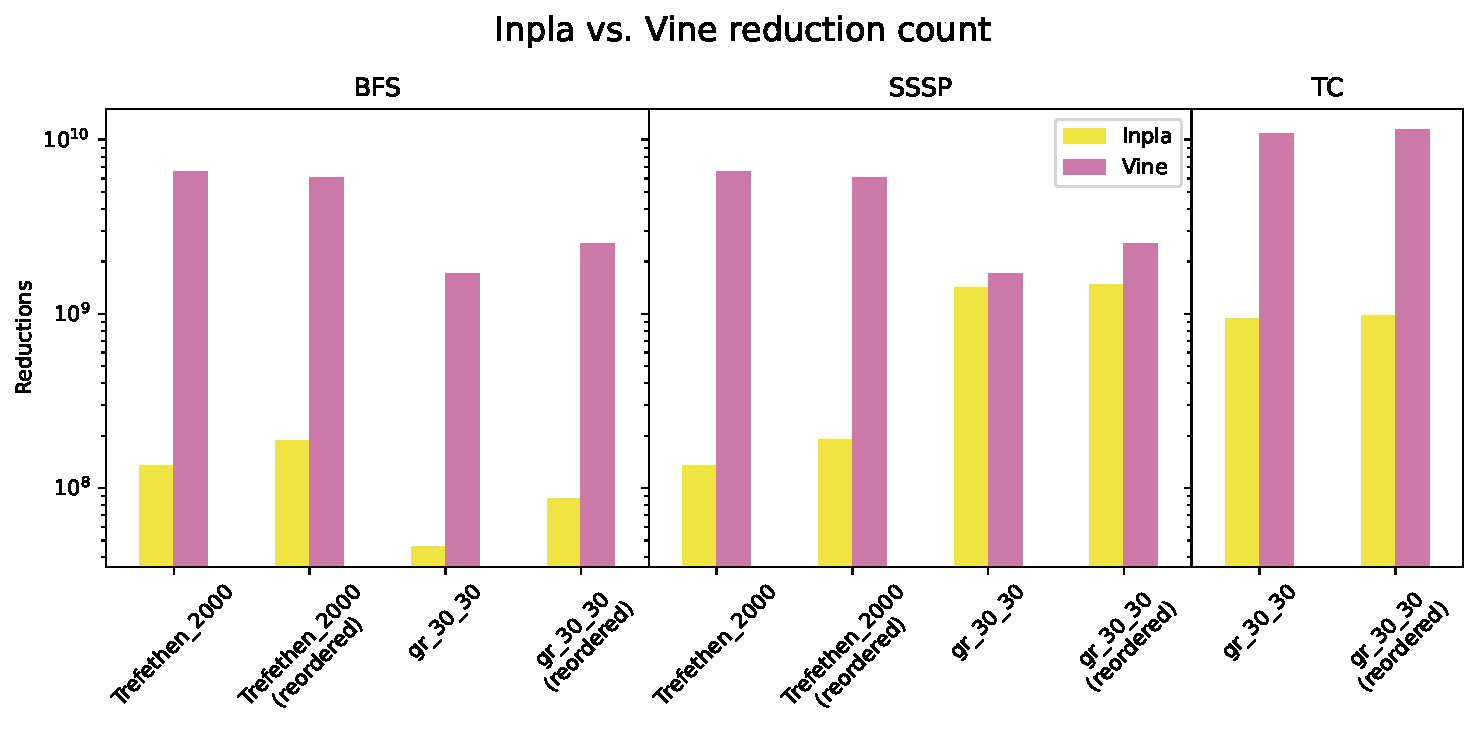
\includegraphics[width=0.39\textwidth]{figures/inpla_vs_vine_reductions_all.pdf}
  \end{center}
  \caption{Total number of interactions}
  \label{fig:total_number_of_interactions}
\end{wrapfigure}
Also we analyze total number of reductions presented in Figure~\ref{fig:total_number_of_interactions}. as expected, Vine performs significantely more reductions because compile code to fixed set of basics agents while Inpla allows user to use custom agents. 
Inpla way can be better to optimize domain-specific computatuions.

To summarize.
\begin{itemize}
    \item Coding patterns together with evaluation strategu=y and memory menegenet mechnisms to reduce memory consumption.
    \item Load balancing (reordering and scaling)
    \item Configuration of Inpla (performance on small graphs)
    \item Anomaly number of reductions and performance for SSSP on \emph{gr\_30\_30} Gap in number of reductions is smaller than in other cases. Performance of Vine is better than Inpla. SSSP only. BSF ok. 
\end{itemize}
\section{Conclusion and Future Work}\label{sec:conclusion}

Summarizing our evaluation, we highlight the following directions for further investigation.

\begin{enumerate}
    \item \textbf{Memory consumption.} Interaction nets programming requires duplicator agents for data reuse. Inpla eagerly copies entire subnets during duplication, incurring substantial memory overhead relative to the F\# prototype. Vine adopts a different strategy but still demands significant memory. Can coding patterns, evaluation strategies, and memory management mechanisms be co-designed to substantially reduce memory consumption?
    
    \item \textbf{Alternative matrix representations.} Tree-based representations looks suboptimal: the recursive divide-and-conquer pattern induces aggressive duplication, traversal dominates cell handling, and performance is highly sensitive to reordering. Could coordinate list (COO) formats~--- operations on which rely on sorting, a task that parallelizes well in interaction nets~--- offer better memory efficiency and performance?
    
   \item \textbf{Load balancing and scaling.} The current configuration of Inpla scales poorly on small graphs but well on large ones. Vine generally scales better than Inpla. Scaling and performance of both tools remain sensitive to matrix reordering. Can the load balancing strategy be improved to address these issues?
    
    \item \textbf{Advanced fusion techniques.} Optimization techniques from functional programming, such as supercompilation~\cite{10.1007/3-540-62064-8_20} or distillation~\cite{10.1007/978-3-030-98869-2_7}, could automate the fusion of operation sequences, analogous to manual kernel fusion for masks and other constructs in SuiteSparse:GraphBLAS. While partial evaluation has been shown possible for interaction nets~\cite{DBLP:conf/sas/Bechet92}, whether these more advanced techniques are adaptable remains an open question.
    
    \item \textbf{FPGA acceleration.} Could an FPGA designed specifically for interaction net reduction exploit the model's fine-grained parallelism, overcome scaling limitations of general-purpose hardware, and achieve substantial performance gains?
\end{enumerate}

Finally, we believe our work motivates comparisons among different interaction net implementations~--- in particular, by extending our evaluation to other systems such as HVM~--- and helps make interaction nets applicable to real-world problems.
%\section{Code Availability Statement}

    F\# prototyping code.

    Inpla implementation.

    Benchmarking scripts and dataset configurations.

%  \section{Appendices}
%  
%  If your work needs an appendix, add it before the
%  ``\verb|\end{document}|'' command at the conclusion of your source
%  document.
%  
%  Start the appendix with the ``\verb|\appendix|'' command:
%  \begin{lstlisting}
%  \appendix
%  \end{lstlisting}
%  and note that in the appendix, sections are lettered, not
%  numbered. 

%%
%% The acknowledgments section is defined using the "acknowledgments" environment
%% (and NOT an unnumbered section). This ensures the proper
%% identification of the section in the article metadata, and the
%% consistent spelling of the heading.
\begin{acknowledgments}
  This research has been supported by the St. Petersburg State University, grant id 116636233.
\end{acknowledgments}

%% The declaration on generative AI comes in effect
%% in Janary 2025. See also
%% https://ceur-ws.org/GenAI/Policy.html
\section*{Declaration on Generative AI}
 %(by using the activity taxonomy in ceur-ws.org/genai-tax.html)
 
 During the preparation of this work, the authors used deepseek in order to: Grammar and spelling check. 
 After using these tool, the authors reviewed and edited the content as needed and take full responsibility for the publication’s content. 

%%
%% Define the bibliography file to be used
\bibliography{GraphBLAS_in_Interaction_Nets}

%%
%% If your work has an appendix, this is the place to put it.
% \appendix
% 
% \section{Online Resources}
% 
% 
% The sources for the ceur-art style are available via
% \begin{itemize}
% \item \href{https://github.com/yamadharma/ceurart}{GitHub},
% % \item \href{https://www.overleaf.com/project/5e76702c4acae70001d3bc87}{Overleaf},
% \item
%   \href{https://www.overleaf.com/latex/templates/template-for-submissions-to-ceur-workshop-proceedings-ceur-ws-dot-org/pkfscdkgkhcq}{Overleaf
%     template}.
% \end{itemize}

\end{document}

%%
%% End of file

